\chapter{Schematy płytek drukowanych}
\label{boards}

\section{Urządzenie deaktywujące}

Ze względu na pełniony przez urządzenie cel, powinno ono zawsze towarzyszyć osobie upoważnionej do uruchomienia pojazdu. Biorąc pod uwagę przykład zastosowania urządzenia we flotach pojazdów, szybko można zauważyć, że zazwyczaj do pojazdu nie jest przypisana jedna osoba, lecz może być on używany przez wielu kierowców. Stąd też logicznym staje się wniosek, że urządzenie nie może być przyporządkowane do kierowcy, lecz do pojazdu. Idealnym rozwiązaniem wydaje się umieszczenie go jako dodatkowy brelok przy kluczykach lub karcie umożliwiającej uruchomienie pojazdu bezkluczykowo. Z tego powodu ważne stają się wymiary samego urządzenia. Nie powinno być ono zbyt grube, aby nie przeszkadzało w kieszeni, ani zbyt duże, aby nie obijało się o nogi, a tym samym nie rozpraszało kierującego w trakcie jazdy.
Wymiary płytki urządzenia deaktywującego wynoszą odpowiednio 32 mm x 43 mm szerokości i wysokości.

Ze względu na prostotę urządzenia, składa się ono z bardzo niewielu modułów.
Na górnej warstwie płytki znajduje się serce układu - mikrokontroler nRF52832 wraz z anteną 2.4 GHz ISM do komunikacji poprzez Bluetooth Low Energy. Dodatkowo, znajdują się tam złącze do programowania, złącze debugowe oraz antena NFC, zwizualizowana jako koło w kolorze niebieskim. Górną warstwę płytki przedstawiono na rysunku \ref{fig:image_key_tag_top_board}.

Centralne miejsce na dolnej warstwie płytki zajmuje bateria litowa CR2032, która zapewni kilkuletnią pracę dezaktywatora. Posiada ona średnicę 20 mm oraz grubość 3.2 mm, co stanowi idealny kompromis pomiędzy wymiarami urządzenia, a czasem jego pracy. Mniejsze baterie oferują mniejszą pojemność liczoną w miliampero godzinach, a także większy opór wewnętrzny co zwiększa straty energetyczne. Wygląd oraz wizualizację dolnej warstwy płytki przedstawiono na rysunku \ref{fig:image_key_tag_bottom_board}.

\begin{figure}[H]
\centering
	\subfloat[Wygląd górnej warstwy płytki]{
		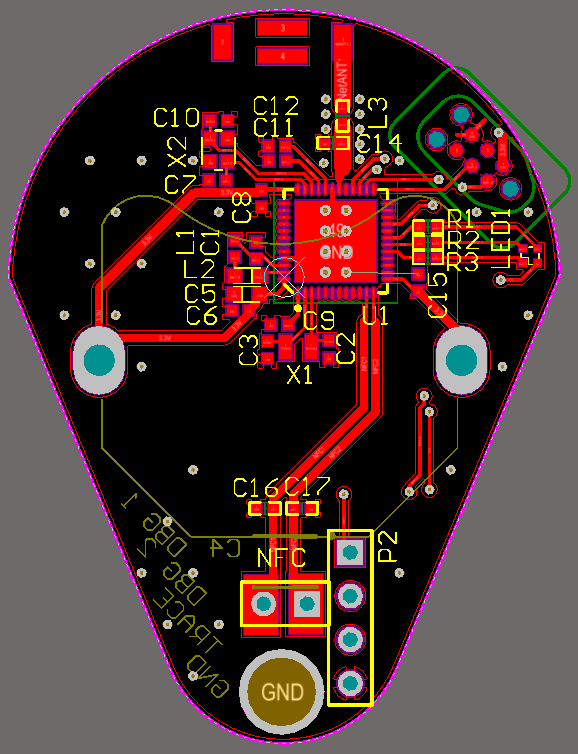
\includegraphics[width=6cm]{img/board_layouts/key_tag_top.png}
	}
	\qquad
	\subfloat[Wizualizacja górnej warstwy płytki]{
		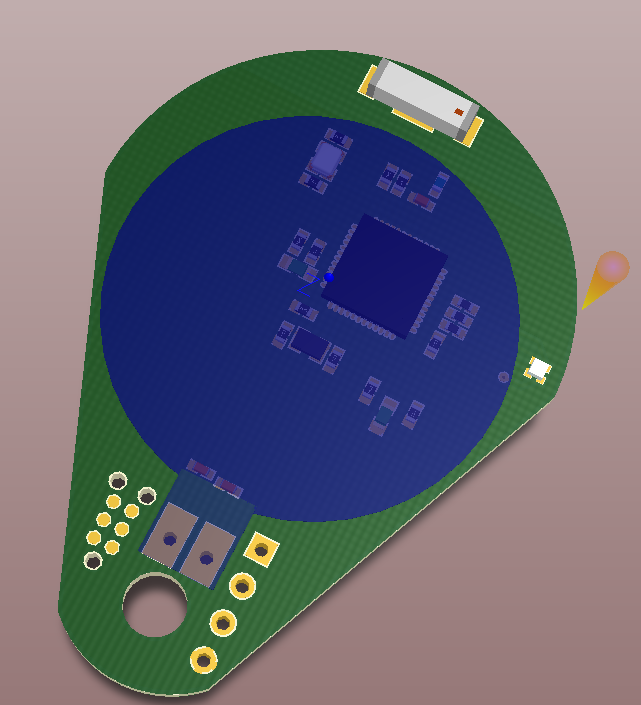
\includegraphics[width=7.1cm]{img/board_layouts/key_tag_visualization_top.png}
	}
	
	\caption{Wygląd górnej warstwy płytki urządzenia deaktywującego oraz jej wizualizacja. \\ Źródło: Twórczość własna}
	\label{fig:image_key_tag_top_board}
\end{figure}

\begin{figure}[H]
\centering
	\subfloat[Wygląd dolnej warstwy płytki]
	{
		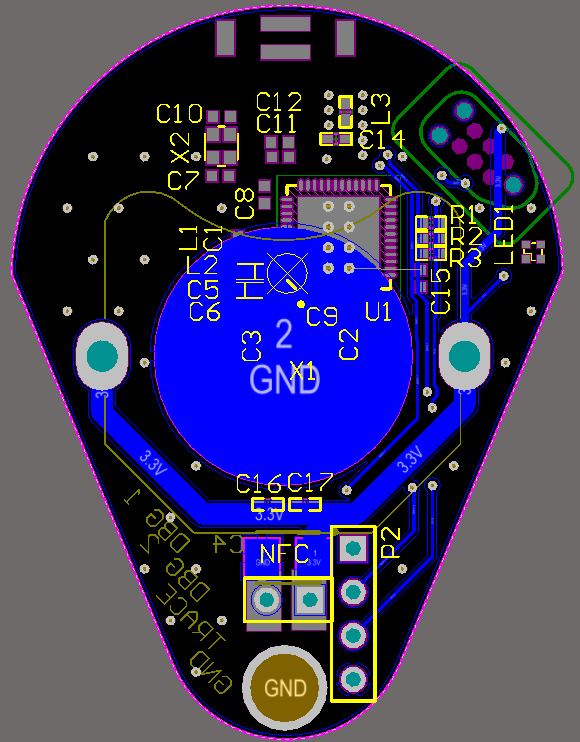
\includegraphics[width=6cm]{img/board_layouts/key_tag_bottom.png}
	}
	\qquad
	\subfloat[Wizualizacja dolnej warstwy płytki]
	{
		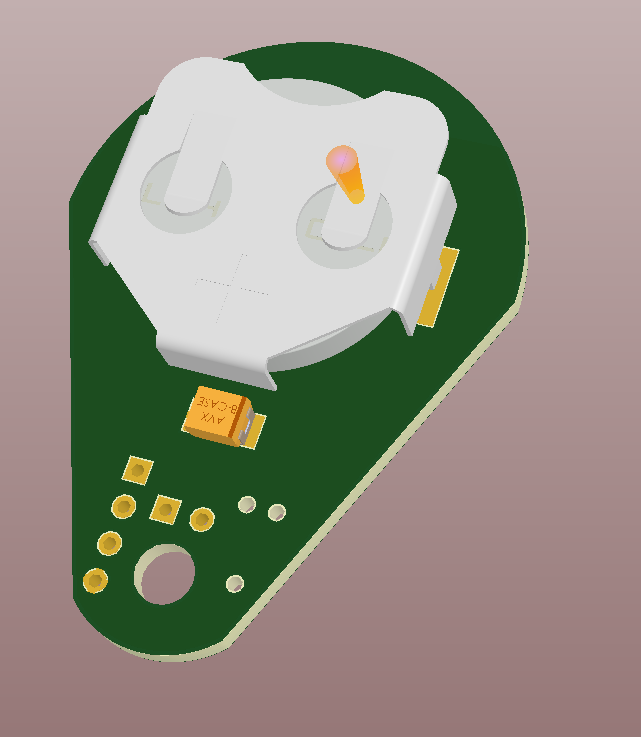
\includegraphics[width=7.1cm]{img/board_layouts/key_tag_visualization_bottom.png}
	}
	
	\caption{Wygląd dolnej warstwy płytki urządzenia deaktywującego oraz jej wizualizacja. \\ Źródło: Twórczość własna}
	\label{fig:image_key_tag_bottom_board}
\end{figure}

\section{Urządzenie lokalizujące}

Płytka lokalizująca jest znacznie bardziej skomplikowana od urządzenia deaktywującego. Wynika to głównie z faktu, iż stanowi podstawę funkcjonalności całego systemu, a zatem posiada wiele modułów realizujących określone zadania. Płytka ma wymiary 50 mm x 50 mm, co powinno umożliwić ukrycie jej w większości miejsc w pojeździe (na przykład pod plastikowymi zabudowami kokpitu). 

Wygląd i wizualizacje urządzenia przedstawiono na końcu tego rozdziału, na rysunkach \ref{fig:image_mainboard_top_board} oraz \ref{fig:image_mainboard_bottom_board}.

Ze względu na użycie kilku układów radiowych, wykorzystujących częstotliwości od 13.56 MHz (NFC), poprzez 900 MHz/ 1800 MHz (GSM) i 1575.42 MHz (GPS) aż po 2.4 GHz (Bluetooth), a także przetwornicy impulsowej o znacznym szczytowym natężeniu prądu (aż do 1.5 A), niezbędne jest odpowiednie rozłożenie elmentów na płytce, które zminimalizowałoby ich wzajemny wpływ. W związku z tym, postanowiono umieścić kluczowe elementy zasilające oraz radiowe w rogach płytki, aby zmaksymalizować wzajemne odległości. W ten sposób, w lewym górnym rogu płytki umieszczono złącza zasilania wejściowego, w prawym górnym - cewkę indukcyjną, stanowiącą główny element impulsowej stabilizacji napięcia. Cewka ta przy okazji stanowi główne źródło zakłóceń sygnałów. W lewym dolnym rogu znajduje się antena Bluetooth Low Energy, natomiast w prawym dolnym rogu - złącze anteny GPS. 

Przewody anten GPS oraz GSM są dodatkowo ekranowane, dzięki czemu znacznie zmniejszona jest podatność tych sygnałów na zakłócenia w trakcie przepływu od anteny do płytki. Jednakże na samej płytce sygnały te nie posiadają ekranu elektromagnetycznego, przez co są podatne na szumy. Z tego względu niezbędna jest minimalizacja długości ścieżek między złączem anteny oraz wejściami układów. W dodatku, sygnał GPS stanowi najsłabszy ze wszystkich sygnałów radiowych, wykorzystywanych w urządzeniu, przez co niezbędne staje się  jak największe oddalenie toru GPS od pozostałych układów. Ze względu na fakt, iż sygnał GSM jest znacznie mocniejszy przez co jest mniej podatny na zakłócenia, jego tor radiowy znajduje się na środku prawego boku płytki, bliżej cewki indukcyjnej przetwornicy impulsowej. 

Wszystkie sygnały radiowe użyte w urządzeniu są sygnałami analogowymi. Są one podatne na zjawisko odbicia fali elektromagnetycznej, które polega na odbiciu sygnału na końcu przewodu, bądź ścieżki elektrycznej i nałożeniu się na sygnał pierwotny. Wprowadza to dodatkowe zakłócenia w transmisji sygnału, a spowodowane jest niedopasowaniem impedancji toru transmisyjnego. Aby zminimalizować ten efekt, należy zaprojektować ścieżki po których przesyłany jest sygnał wysokiej częstotliwości tak, aby miały odpowiednią impedancję, zgodną z impedancją anteny. Dokonuje się to poprzez dobór grubości (wynika ona z grubości warsty miedzi, zazwyczaj 35 $\mu m$) oraz szerokości (wybór pod kątem optymalności zużycia miejsca na PCB) ścieżek radiowych. Na podstawie tak wyznaczonych parametrów wylicza się ich niezbędną długość, aby osiągnąć założoną impedancję. W przypadku sygnałów GPS, GSM oraz Bluetooth wynosi ona 50 $\Omega$. Ostateczną impedancję, uwzględniającą pojemności i indukcyjności pasożytnicze między ścieżkami, zmierzoną po złożeniu płytki można jeszcze skorygować poprzez dobór elementów w filtrach przyantenowych (filtry: C45, R21, C47 oraz C44, R22, C46). Dodatkowo, ścieżki wysokiej częstotliwości prowadzi się łagodnymi łukami, bez ostrych załamań, które mogłyby zwiększających pojemność, a tym samym mogących zmienić impedancję. 

W dodatku, w trakcie projektowania urządzenia należy pamiętać o wysokim chwilowym poborze prądu (aż do około 2 A). Z tego względu, trzeba zaprojektować odpowiednio grube ścieżki zasilające. Jest to wymagane z dwóch powodów. Pierwszym z nich jest fakt oporności ścieżki.

\begin{equation}
 R = \rho \cdot l / S 
 \label{eq_pcb_wire_resistance}
\end{equation}

gdzie:

R - oporność ścieżki,

$\rho$ - oporność właściwa materiału, z którego wykonano ścieżkę,

l - długość ścieżki,

S - powierzchnia (liczona jako iloczyn grubości i szerokości) ścieżki,

Jak widać, im większa szerokość ścieżki, tym większa jej powierzchnia, a więc mniejsza rezystancja. Im mniejsza rezystancja, tym straty napięcia na samej ścieżce będą mniejsze, a tym samym większe napięcie dostarczane do układów funkcjonalnych i mniejsze straty na ciepło, generujące niepotrzebne zużycie energii.

\begin{equation}
 U = R \cdot I
 \label{eq_voltage_drop_on_pcb_wire} 
\end{equation}

 gdzie:
 
 U - strata napięcie na ścieżce,
 
 R - opór ścieżki,
 
 I - prąd płynący przez ścieżkę
 
\clearpage
Drugi przypadek wynika niejako z pierwszego. Gdy opór ścieżki jest zbyt duży, w momencie zwiększonego poboru prądu, energia tracona na ścieżce może być tak duża, że ulega ona przepaleniu i całe urządzenie przestaje działać. Aby się przed tym ustrzec, ścieżki zasilające mają grubość 2 mm, co pozwala na przepływ około 3.5 A nateżęnia ciągłego prądu w temperaturze 20 stopni Celsjusza. Ze względu jednak na fakt, iż główne obciążenie urządzenia stanowi prąd chwilowy, trwający bardzo krótko, średnie natężenie prądu będzie dużo niższe od tej wartości. Szerokość ścieżek została dobrana z zapasem, aby nie uległy one przepaleniu przed zadziałaniem bezpiecznika zwłocznego i zmniejszyć straty energii. Tabela zestawiająca zależność między grubością ścieżek na płytce PCB od wartości maksymalnego dopuszczalnego prądu ciągłego, przepływającego przez nią, przedstawiono na rysunku \ref{fig:image_pcb_wire_thickness}.

\begin{figure}[H]
	\centering
	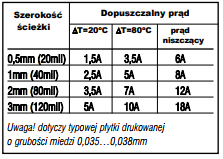
\includegraphics[width=6cm]{img/board_layouts/pcb_wire_thickness.png}
	\caption{Tabela opisująca korelację między grubością ścieżek, a maksymalnym dopuszczalnym natężęniem prądu. Źródło: \cite{pcb_wire_thickness}}
	\label{fig:image_pcb_wire_thickness}
\end{figure}
 

\begin{figure}[H]
\centering
	\subfloat[Wygląd górnej warstwy płytki]{
		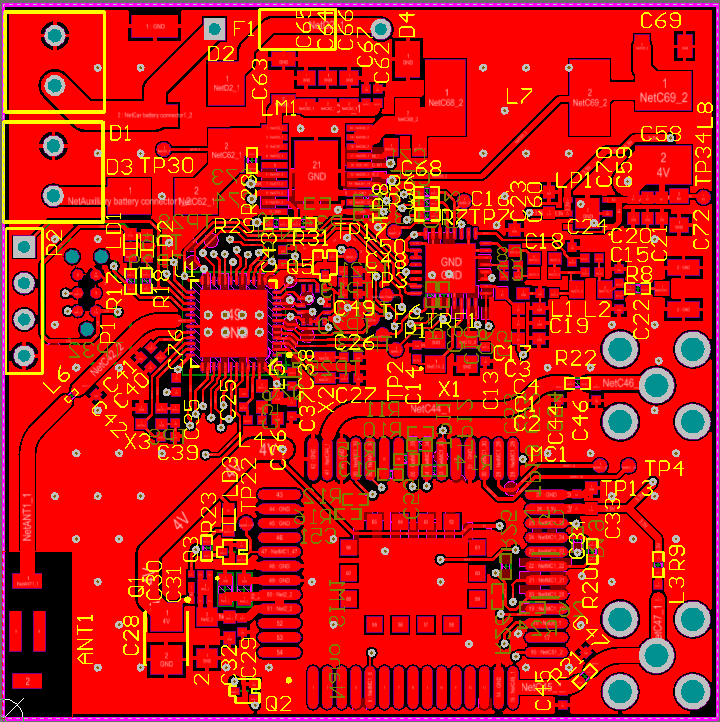
\includegraphics[width=11cm]{img/board_layouts/mainboard_top.png}
	}
	\qquad
	\subfloat[Wizualizacja górnej warstwy płytki]{
		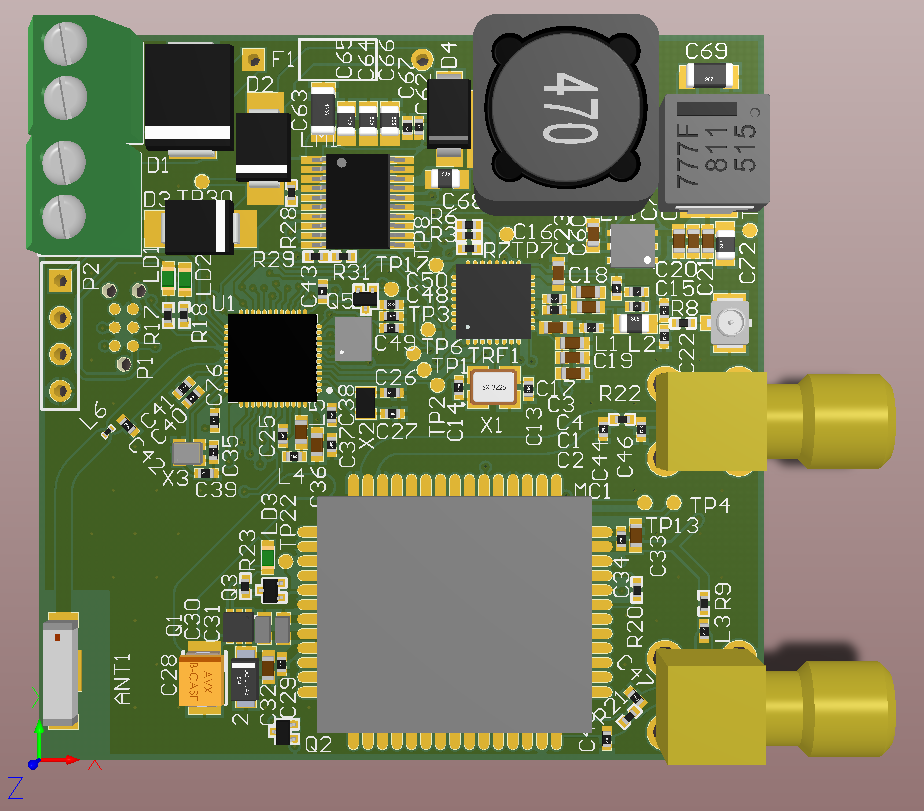
\includegraphics[width=11cm]{img/board_layouts/mainboard_visualization_top.png}
	}
	
	\caption{Wygląd górnej warstwy płytki urządzenia lokalizującego oraz jej wizualizacja. \\ Źródło: Twórczość własna}
	\label{fig:image_mainboard_top_board}
\end{figure}

\begin{figure}[H]
\centering
	\subfloat[Wygląd dolnej warstwy płytki]
	{
		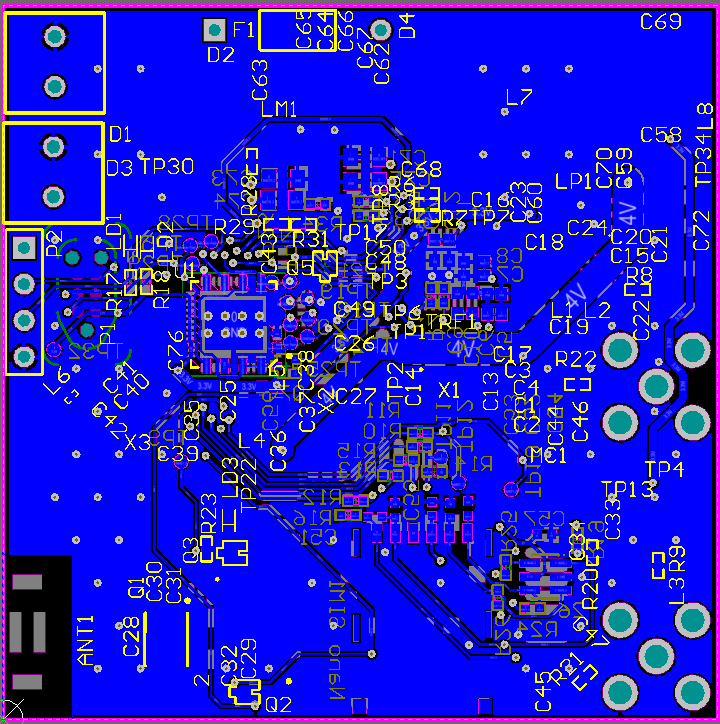
\includegraphics[width=11cm]{img/board_layouts/mainboard_bottom.png}
	}
	\qquad
	\subfloat[Wizualizacja dolnej warstwy płytki]
	{
		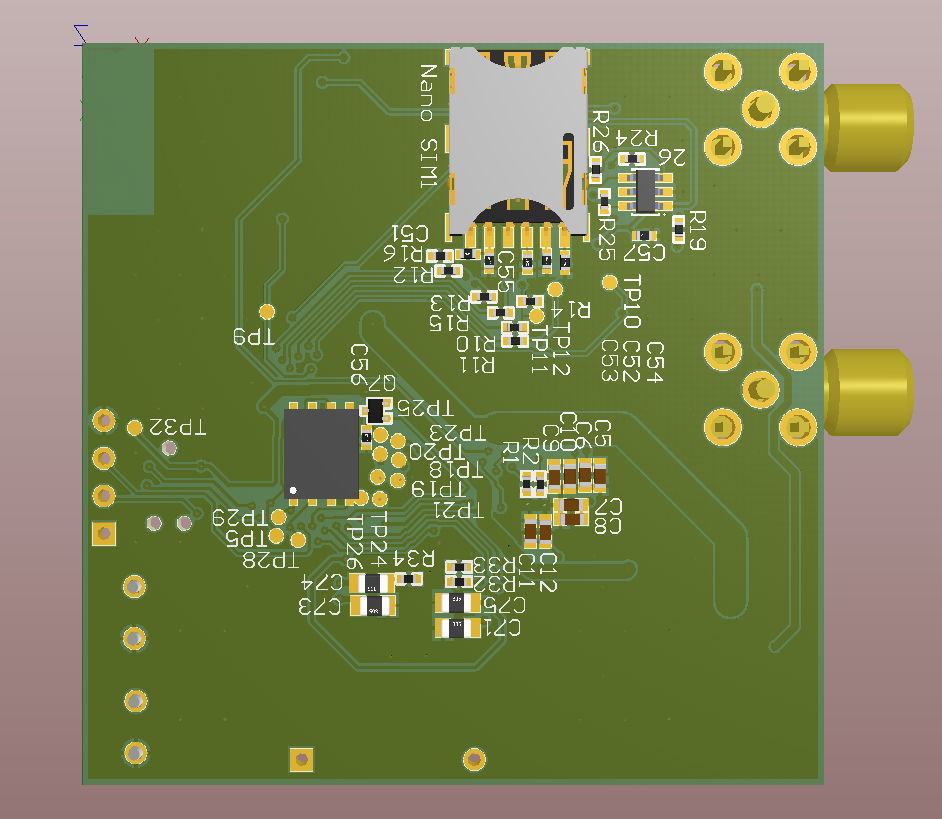
\includegraphics[width=11cm]{img/board_layouts/mainboard_visualization_bottom.png}
	}
	
	\caption{Wygląd dolnej warstwy płytki urządzenia lokalizującego oraz jej wizualizacja. \\ Źródło: Twórczość własna}
	\label{fig:image_mainboard_bottom_board}
\end{figure}